\subsection{A string representation for our memory box}
\begin{figure}[htbp]
\begin{center}
  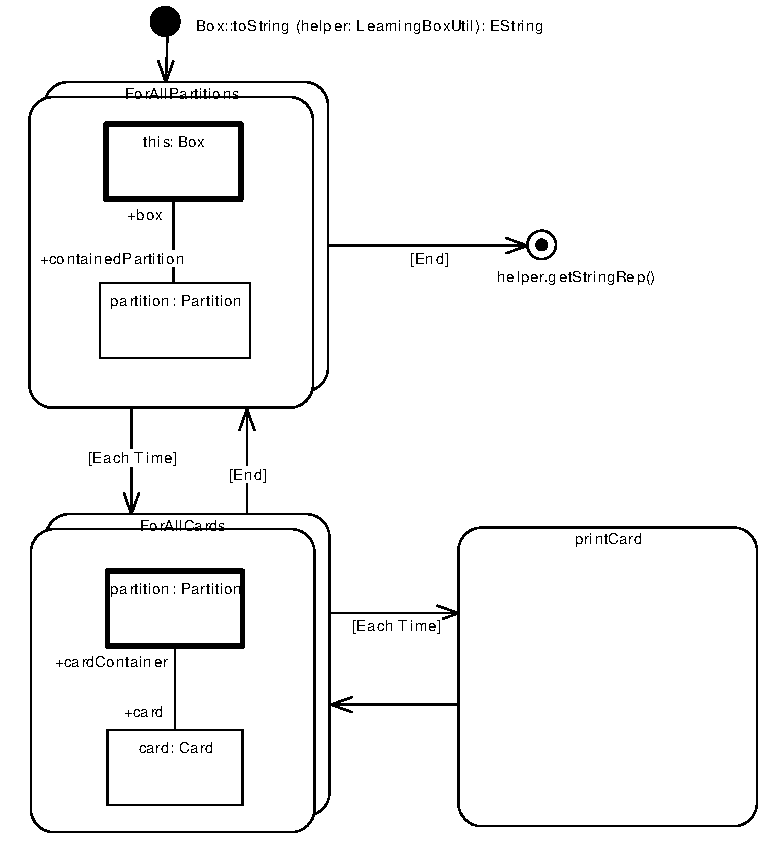
\includegraphics[width=0.7\textwidth]{pics/sdmBilder/toString/sdm72}
  \caption{Control flow with nested loops.}  
  \label{fig:sdm_invert_1}
\end{center}
\end{figure}

\begin{figure}[htbp]
\begin{center}
  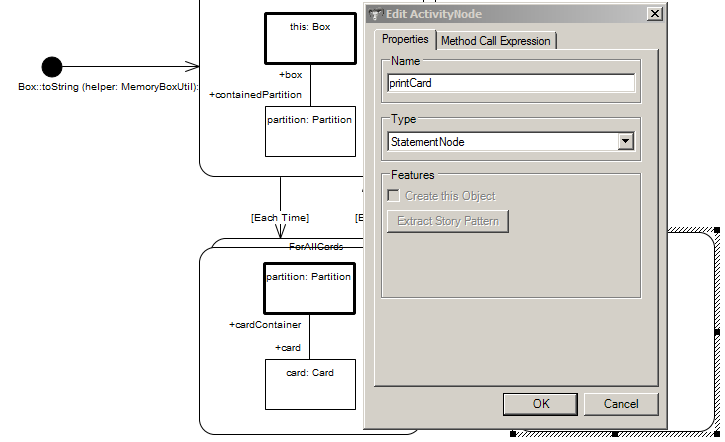
\includegraphics[width=0.7\textwidth]{pics/sdmBilder/toString/sdm73}
  \caption{Invoking a method in a \texttt{StatementNode}.}  
  \label{fig:sdm_invert_2}
\end{center}
\end{figure}

\begin{figure}[htbp]
\begin{center}
  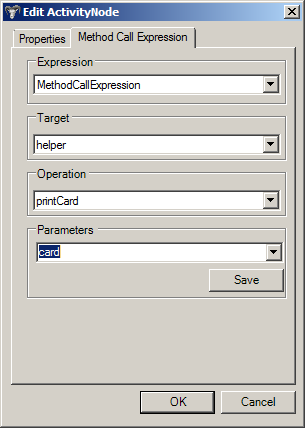
\includegraphics[width=0.5\textwidth]{pics/sdmBilder/toString/sdm74}
  \caption{Specify a \texttt{MethodCallExpression} in the
  \texttt{StatementNode}.}
  \label{fig:sdm_invert_3}
\end{center}
\end{figure}

\begin{figure}[htbp]
\begin{center}
  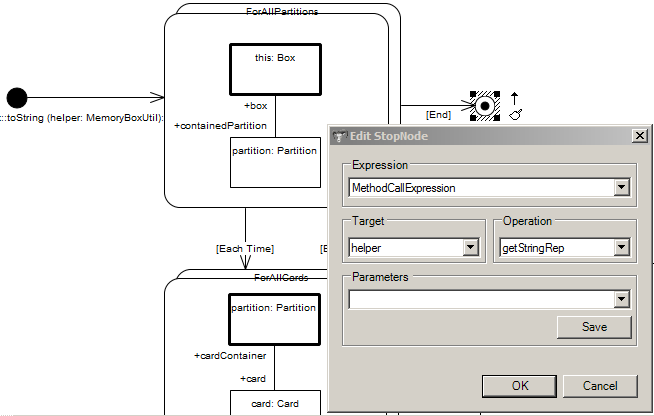
\includegraphics[width=0.7\textwidth]{pics/sdmBilder/toString/sdm75}
  \caption{Using a \texttt{MethodCallExpression} as a return value.}  
  \label{fig:sdm_invert_4}
\end{center}
\end{figure}

\begin{figure}[htbp]
\begin{center}
  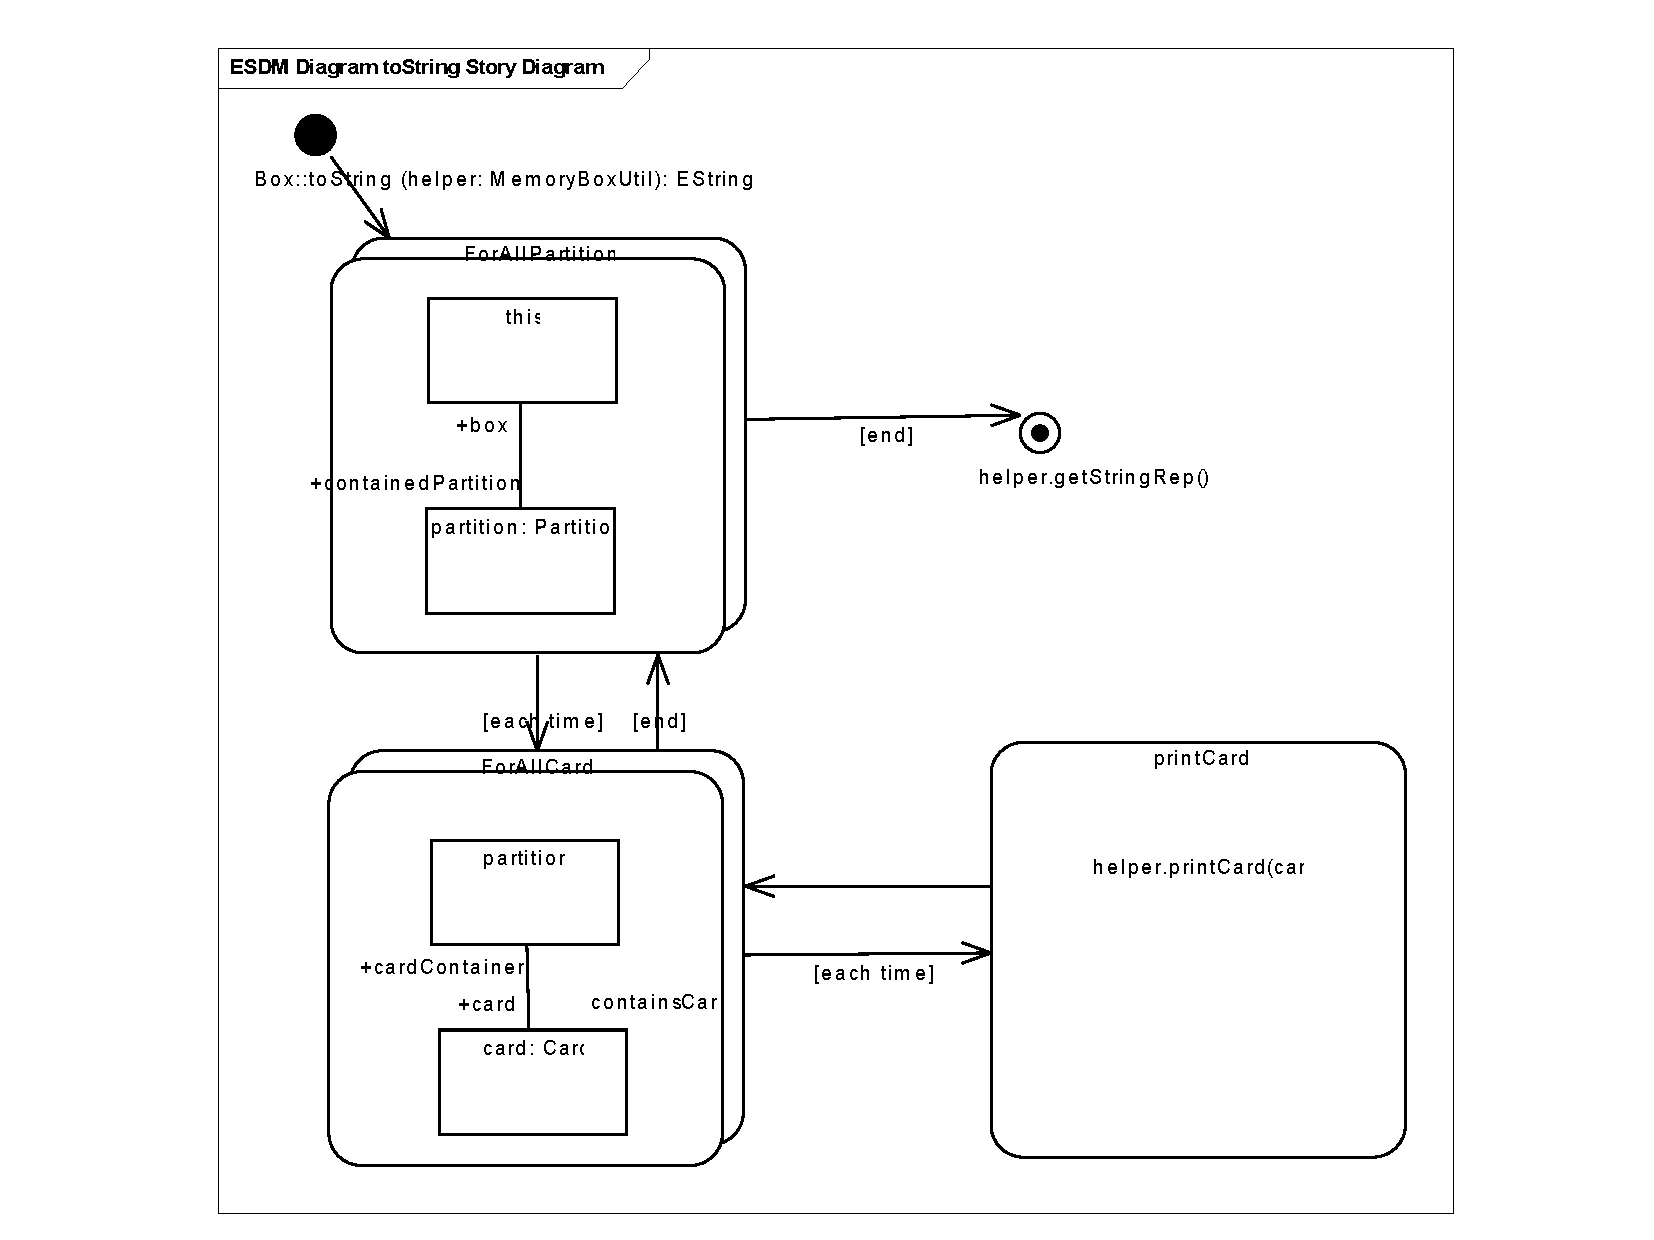
\includegraphics[width=0.7\textwidth]{pics/sdmBilder/toString/sdm76}
  \caption{The complete SDM for \texttt{Box::toString}.}  
  \label{fig:sdm_invert_5}
\end{center}
\end{figure}

\clearpage 